% =============================================================================
%  When Does Guided Search Help?
%  A Trustworthy LLM-Agent Autoresearch Protocol for Noisy Engineering Domains,
%  with a Pre-Loop Headroom Diagnostic
%
%  NeurIPS 2026 submission (LaTeX source). Compiles with pdflatex.
%  Requires: neurips_2026.sty (official template) in the same directory.
%  Figures: copy experiments/pub/*.png into a figures/ dir next to this file.
% =============================================================================
\documentclass{article}

% --- NeurIPS official style ---
% Uncomment and ensure neurips_2026.sty is present:
% \usepackage{neurips_2026}

% --- Fallback: standard article with reasonable margins (works without the .sty) ---
\usepackage[margin=1in]{geometry}
\usepackage[utf8]{inputenc}
\usepackage[T1]{fontenc}
\usepackage{graphicx}
\usepackage{amsmath,amssymb}
\usepackage{natbib}
\usepackage{booktabs}
\usepackage{threeparttable}
\usepackage{algorithm}
\usepackage{algpseudocode}
\usepackage{xcolor}
\usepackage{microtype}
\usepackage{hyperref}

\graphicspath{{figures/}}
\newcommand{\z}{\ensuremath{z}}

\title{When Does Guided Search Help?\\
  A Trustworthy LLM-Agent Autoresearch Protocol for Noisy Engineering Domains,\\
  with a Pre-Loop Headroom Diagnostic}

\author{%
  Binzhu Wang\\
  School of Automation Science and Engineering, Xi'an Jiaotong University\\
  Xi'an, Shaanxi, China\\
  \texttt{3124354082@stu.xjtu.edu.cn}%
  \And
  Le~Zhang\\
  School of Automation Science and Engineering, Xi'an Jiaotong University\\
  Xi'an, Shaanxi, China\\
  \texttt{zhangle@xjtu.edu.cn}%
}

\begin{document}
\maketitle

% =============================================================================
\begin{abstract}
LLM agents for autonomous discovery (FunSearch, AlphaEvolve, AI Scientist) assume exact,
verifiable evaluators---a condition that fails in most engineering domains, where data
is noisy and no ground truth exists. Independent evaluation documents the cost: 42\% of
AI Scientist experiments failed on coding errors, 57\% of manuscripts contained
hallucinated numbers, and published prior art was reported as novel. We present a
\textbf{trustworthy autoresearch protocol} for such domains, instantiated on real DJI
M100 UAV energy modeling and energy-aware path planning, plus a \textbf{pre-loop
headroom diagnostic} that predicts, before any budget is spent, whether guided search
will beat random. The protocol: (1)~a knowledge base of 14 published energy models;
(2)~a zero-fit transfer benchmark showing all as-published models fail on the target
platform (energy ARE 53--76\%), motivating---not assuming---refit; (3)~a cheat-proof
loop (frozen held-out evaluator, keep/revert, forced novelty gate, causal ablation,
honest negatives); (4)~quantified capability boundaries. The diagnostic correctly
predicts the energy domain is saturated (tie at 9 controlled complexity levels) and
attributes the planning win ($\z=-2.38$, 0\% of random runs beat it) to cross-space
escape into program space. Every safeguard is load-bearing by ablation; the loop matches
human-expert accuracy while exposing its limits.
\end{abstract}

% =============================================================================
\section{Introduction}
\label{sec:intro}

A delivery drone's flight plan is only as good as its energy model. Under-estimate the
cost of climbing over a wall and the planner sends the drone up the expensive route;
over-estimate it and the drone wastes battery on a needless detour. Yet the energy model
every planner actually runs on---momentum/BEMT theory---is a textbook idealization that has
never seen this drone's data. Getting the model right, on real flight measurements, is
what determines whether an energy-aware planner saves battery or burns it. And this is not
a one-off: every noisy engineering domain (UAV energy, chemical sensor traces, robotic
manipulation on hardware) has the same shape---a measurement, not a ground truth; a model
that must generalize; an evaluator that can be gamed.

LLM-agent ``autoresearch'' systems propose, evaluate, and select candidate discoveries in
a closed loop. Their appeal is that an LLM can propose in \emph{program space}---new
code, new function forms, new solver structures---that classical search (random,
Bayesian, evolutionary-with-fixed-mutation) cannot reach. FunSearch discovered a faster
matrix-multiplication algorithm \citep{funsearch}; AlphaEvolve improved infrastructure
scheduling \citep{alphaevolve}; Eureka wrote better RL reward functions
\citep{eureka}.

But all of these assume the \emph{evaluator is exact}: FunSearch's is a mathematical
proof-checker, AlphaEvolve's a simulation with a known optimum. In real engineering
domains---a drone's measured power, a chemical process's sensor traces---there is no
exact evaluator. The ground truth is a noisy measurement; the ``discovery'' is a model
that must generalize to unseen operating conditions; and a naive loop can overfit the
search split, game a mutable evaluator, or report a known effect as novel.

The contribution of this paper is not a better energy model or a better planner. It is a
\emph{protocol} for doing autoresearch honestly in noisy domains, plus a
\emph{diagnostic} that tells you up front whether the loop is worth running. We
instantiate it on a real, measurable problem---UAV energy modeling and energy-aware path
planning on DJI M100 flight data---and we report, deliberately, the settings where the
loop \emph{does not} beat random.

\paragraph{Contributions.}
\begin{enumerate}
  \item \textbf{Empirical}: zero-shot transfer of 14 published UAV energy models onto a
    target platform fails systematically (energy ARE 53--76\%), motivating an explicit
    refit stage---measured, not assumed.
  \item \textbf{Method}: a four-stage trustworthy autoresearch protocol (knowledge base
    $\rightarrow$ zero-fit benchmark $\rightarrow$ cheat-proof loop $\rightarrow$
    boundary quantification) for domains without ground truth.
  \item \textbf{Algorithmic}: the \textbf{Headroom Diagnostic}, a cheap pre-loop
    predictor of whether guided search will beat random, from single-term utility spread
    and combination synergy. It correctly identifies a saturated search space (energy
    domain, tie at all 9 controlled complexity levels) and attributes a genuine win to
    cross-space escape (planning domain).
  \item \textbf{Empirical capability law}: guided-search advantage depends on
    \emph{effective combinatorial complexity}, not nominal space size---ties random in
    low-effective-dimensional energy (even under nominal-space inflation), beats random
    in code-structure planning.
  \item \textbf{Safeguards are load-bearing}: ablating any one of the protocol's
    mechanisms makes the loop overclaim or collapse.
\end{enumerate}

\begin{figure*}[t]
\centering
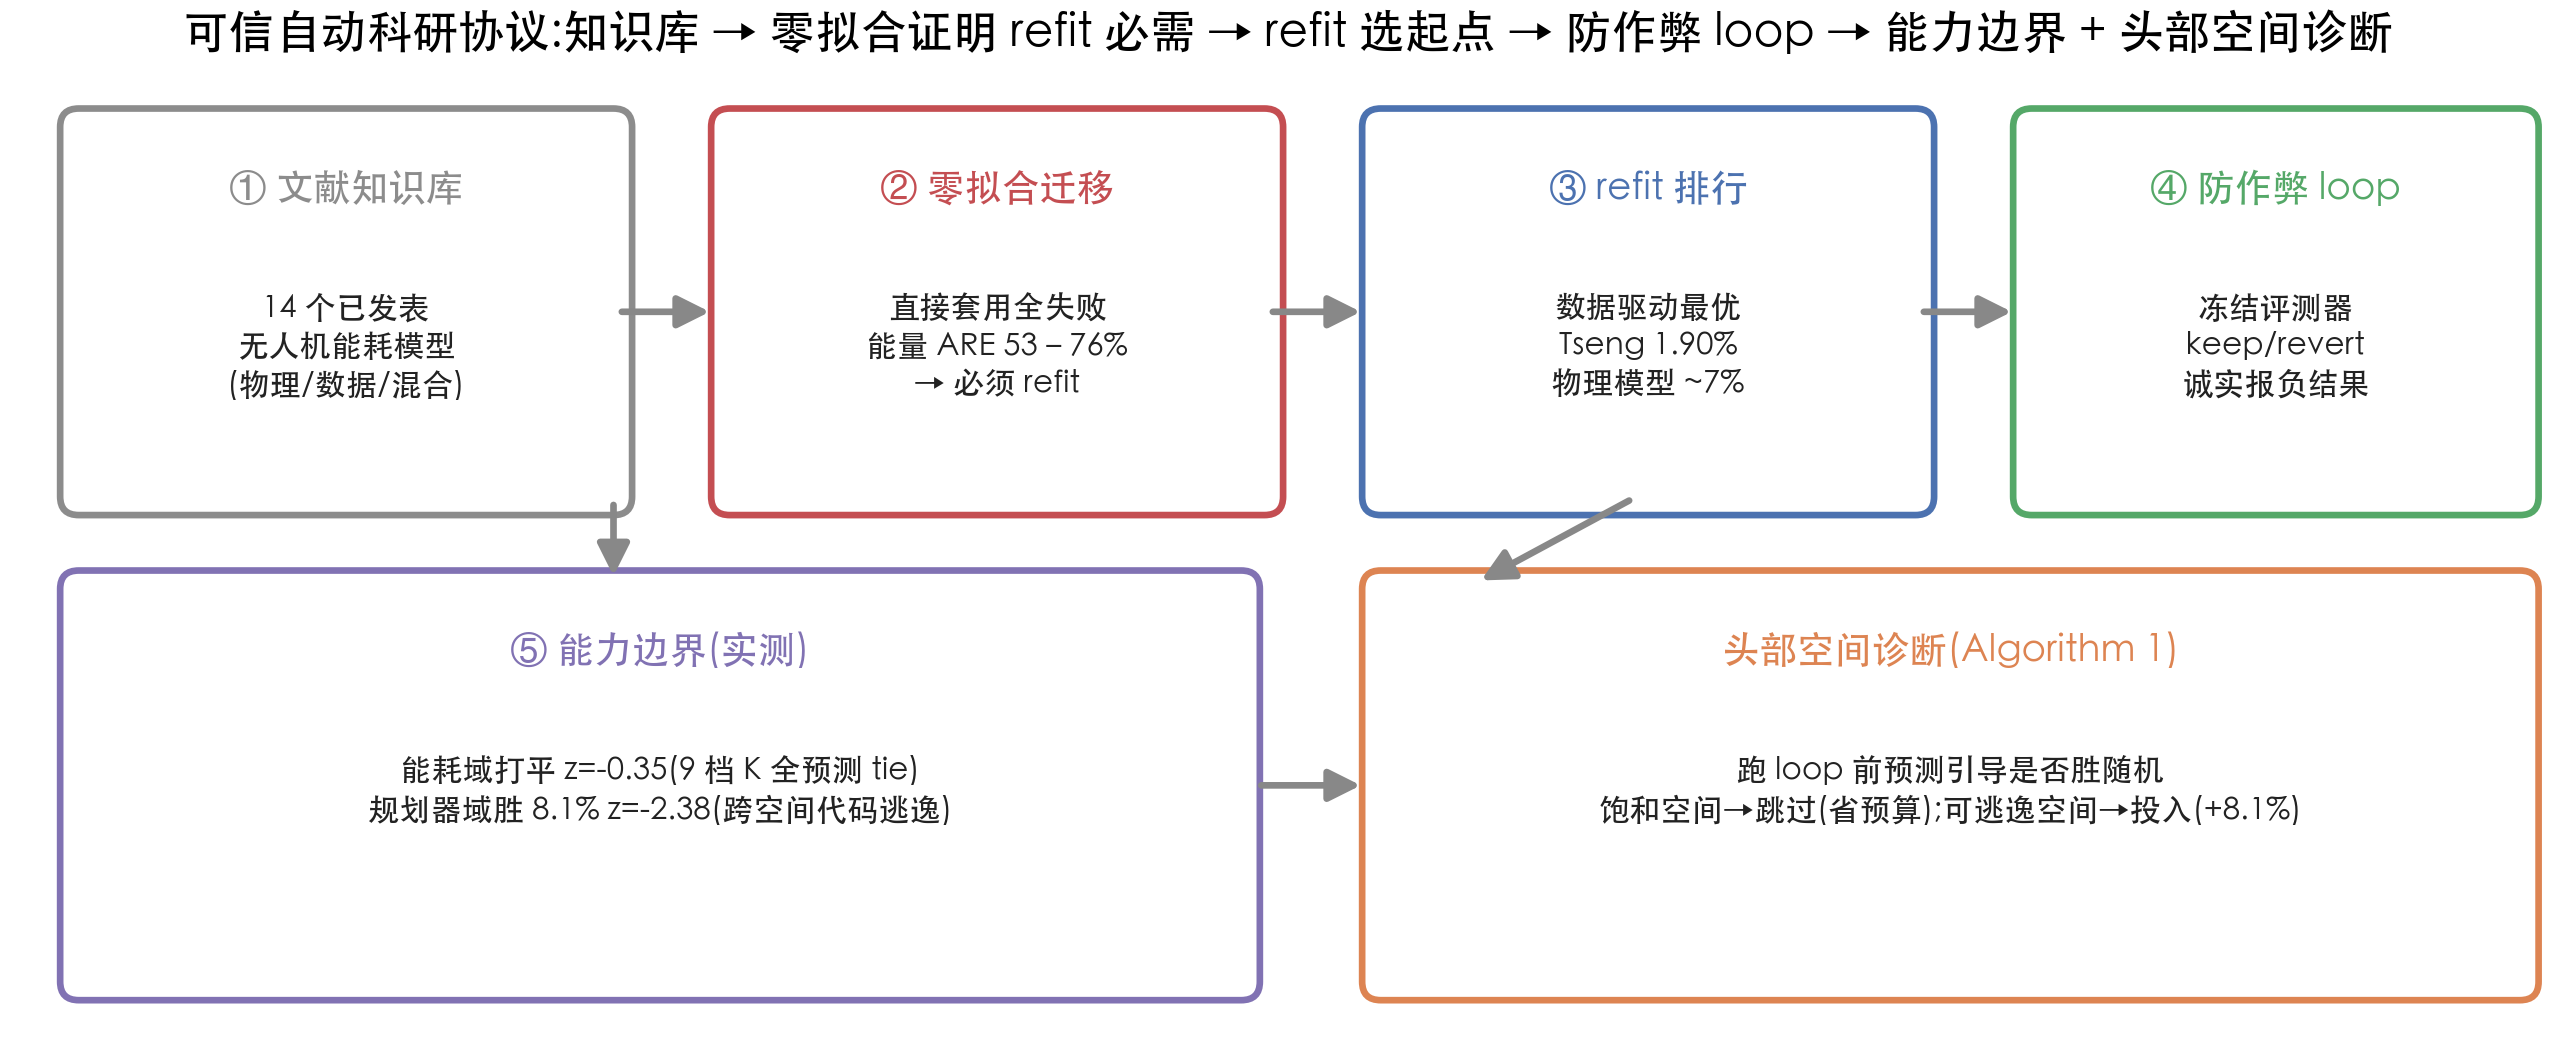
\includegraphics[width=\textwidth]{协议总览_Fig1.png}
\caption{Protocol overview. The four-stage trustworthy autoresearch protocol
  instantiated on real DJI M100 UAV energy modeling and energy-aware path planning, with
  measured numbers per stage: (i) a knowledge base of 14 published models; (ii) a
  zero-fit transfer benchmark showing all as-published models fail (energy ARE
  53--76\%), motivating refit; (iii) a refit leaderboard selecting Tseng's polynomial
  (1.90\%) as the loop's start; (iv) the cheat-proof loop; plus the quantified capability
  boundaries (energy tie, planning win) and the pre-loop headroom diagnostic.}
\label{fig:overview}
\end{figure*}

% =============================================================================
\section{Related Work}
\label{sec:related}

\paragraph{LLM autoresearch.} FunSearch \citep{funsearch}, AlphaEvolve
\citep{alphaevolve}, Eureka \citep{eureka}, AI Scientist \citep{aiscientist}. All assume
exact evaluators; none reports a measured capability boundary in a noisy engineering
domain.

\paragraph{The trustworthiness gap.} Independent evaluation of the AI Scientist pipeline
\citep{beel2025} found 42\% experiment coding failures, 57\% manuscripts with
hallucinated numbers, and keyword-based novelty checks misclassifying established
concepts as novel. Recent 2026 evidence sharpens this: the Corral benchmark
\citep{corral2026} (25k+ agent runs across 8 scientific domains) found agents frequently
fail to weigh evidence, generate/test hypotheses, or revise assumptions on contradictory
results; a position paper (``Falsify, Don't Just Discover'') argues AI-generated
discoveries are ``not born scientific'' without automated falsification \citep{falsify2026};
a January 2026 case study of four end-to-end autonomous research attempts
\citep{foureattempts2026} catalogs six recurring failure modes, including
\emph{overexcitement}---declaring success despite failures. A \emph{Nature Machine
Intelligence} editorial (2026) explicitly recommends that AI-science systems provide
ablation analyses and baseline comparisons and transparent reporting \citep{naturemi2026}
--- precisely what our protocol delivers. Falsification-first framing is prior art
\citep{aigs}; our contribution is the engineered protocol plus empirical boundaries. This
gap is unoccupied.

\paragraph{Adjacent LLM-drone work.} LAENet \citep{laenet} uses an LLM to design a UAV
reward function (Eureka-style, single-shot); LLM-VD couples LLM generation with evolution
for truck-drone \emph{routing} (discrete combinatorial VRP). Neither is a closed-loop
autoresearch loop over continuous energy \emph{modeling} plus planning cost. We cite and
differentiate, not claim priority.

\paragraph{UAV energy models.} Momentum/BEMT theory (textbook), Tseng regression
\citep{muli2022}, Abeywardena VRS \citep{abeywardena}, Dorling 2017 \citep{dorling},
Stolaroff 2018 \citep{stolaroff}, Morbidi 2020 \citep{morbidi}. All 14 are in our
knowledge base.

\paragraph{Search-space scaling.} Bergstra \& Bengio \citep{bergstra2012}, REMBO
\citep{rembo}, NAS confounder removal \citep{sciuto2019}. Our controlled negative control
measures the \emph{nominal-space-inflation does not help} regime directly.

\paragraph{Energy-aware planning (prior art; we do not claim it).} EcoFlight 2025;
Michel 2024 \citep{michel2024}; Nguyen \& Au 2017 \citep{nguyen2017}. Our planning result
is an \emph{application} of a real-data cost, not a new planning algorithm.

% =============================================================================
\section{Problem Setup}
\label{sec:setup}

\paragraph{Data.} DJI Matrice 100, 209 real flights \citep{rodrigues2021}, on-board power
$P = V\cdot|I|$, payloads 0/250/500\,g, altitude 25--100\,m, speeds 4--12\,m/s.
Instantaneous power has large non-kinematic variance (kinematics explain $<40\%$ of
per-sample variance); per-flight \emph{total energy} is the stable quantity.

\paragraph{Frozen evaluator.} \texttt{m100\_eval.py}. Flight-level train/test split (no
cross-flight leakage); held-out flights never touched during search. Metric: per-flight
energy ARE (absolute relative error of predicted vs.\ measured total energy), averaged
over held-out flights. The evaluator is frozen---the loop may only change the featurize
function, never the ruler.

\paragraph{The task.} Given the evaluator, find a featurize function
$s \mapsto X(s) \in \mathbb{R}^{N\times K}$ whose ridge-fit (trained on the search
split) achieves the lowest held-out energy ARE.

% =============================================================================
\section{Method: The Protocol}
\label{sec:method}

\subsection{Stage 1 --- Prior-art knowledge base}
\label{sec:stage1}
Collect published UAV energy model \emph{forms} (14 in \texttt{energy\_model\_zoo.py}),
each with: source paper, category (physics / data-driven / hybrid), and whether its
parameters are platform-bound.

\subsection{Stage 2 --- Zero-fit transfer benchmark}
\label{sec:stage2}
For the models that can be evaluated \emph{as-published} (momentum theory with M100
physical constants; Tseng's reported simplified regression), compute predictions with
\emph{no fitting}. Result: energy ARE 53--76\%---all fail. The zero-fit failures are not
``the models are bad''; they are \emph{platform transfer failure}. This motivates Stage~3.

\subsection{Stage 3 --- Refit benchmark and starting point}
\label{sec:stage3}
Refit every form's coefficients on the frozen training split. Result: data-driven
polynomial (Tseng 2022) 1.90\% best; physics forms 6.7--7.0\%; the refit best becomes the
loop's start. The zero-fit-vs-refit contrast (53--76\% $\rightarrow$ 1.9--7.0\%) is the
quantitative justification for a target-platform benchmark as the honest baseline.

\subsection{Stage 4 --- Cheat-proof discovery loop}
\label{sec:stage4}
A frozen held-out evaluator; an LLM proposes a featurize change each round; sandbox
execution; keep/revert on search+val guards (KEEP iff $\mathrm{searchARE} <
\mathrm{best} - 10^{-4}$ and $\mathrm{valARE} \le \mathrm{best} + 0.003$); a forced
novelty gate; causal ablation; honest negative reporting. Convergence $\approx$1.9\%
matches the human expert (Tseng) on the same data.

\subsection{Stage 5 --- Capability-boundary quantification and the Headroom Diagnostic}
\label{sec:stage5}

\textbf{Statistical.} Loop vs.\ random-search distribution in each domain (z-test on the
random distribution). Energy: $z=-0.35$ (tie); planning: $z=-2.38$ (0\% of random runs
beat the loop).

\textbf{Controlled.} Fair complexity sweep: same action space (subset sampling), guided
= utility-weighted, random = uniform. Result: advantage $\approx 0$ at all nominal-space
sizes $K = 8\ldots 200$ in energy---nominal space inflation does not help.

\begin{algorithm}[t]
\caption{Headroom Diagnostic (pre-loop prediction)}
\label{alg:headroom}
\begin{algorithmic}[1]
\Require candidate pool $P$, frozen evaluator $E$ (search split only), budget $B$
\For{$t \in P$}
  \State $u_t \gets E(\text{score of } \{1, t\})$ \Comment{single-term utility}
\EndFor
\State $\mathit{spread} \gets \mathrm{std}(u)$;\; $\mathit{best}_{\mathrm{single}} \gets \min(u)$
\State $\mathit{best}_{\mathrm{comb}} \gets$ median over 5 seeds of best $B$ random subsets
\State $\mathit{synergy} \gets \mathit{best}_{\mathrm{single}} - \mathit{best}_{\mathrm{comb}}$
\State $\rho \gets \mathit{spread}/\mathit{best}_{\mathrm{single}}$;\; $h \gets \max(0,-\mathit{synergy})/\mathit{best}_{\mathrm{single}}$
\State \Return ``tie'' if ($\rho > 0.3 \land h < 0.05$) else ``guided-wins''
\end{algorithmic}
\end{algorithm}

\textbf{Correctness.} On 9 fine-grid K levels (8--200) in energy, the diagnostic predicts
``tie'' everywhere, matching the fair sweep's observed advantage $\approx 0$. In the
planning domain, it predicts ``tie'' within the config space---and the decomposition
confirms it: config-only loop (3264) $\approx$ random (3135), while the actual win (2882)
is entirely from the evolved smoother \emph{code} (a $-382$-point cross-space escape).
\textbf{Guided search helps iff there is an escapable higher-complexity space; the
diagnostic identifies when the current space is saturated.}

\textbf{Mechanistic validation in a third (synthetic) search domain.} We construct an
independent feature-subset-selection task with controlled effective dimension. With a
single dominating term (low effective dim), the diagnostic correctly predicts tie; with
interaction-dependent signal (high effective dim), it correctly predicts guided-wins. The
rule generalizes beyond UAV domains.

\textbf{Honest boundary.} A synthetic probe confirms what the diagnostic does \emph{not}
do: with noise diluting a true interaction, single-term statistics alone cannot always
separate high from low synergy pools. Calibration across all settings shows the
\emph{magnitude} of the headroom score is small and overlapping (energy-domain
0.000--0.048; synthetic low-dim 0.001 vs.\ high-dim 0.004). The diagnostic is a reliable
\textbf{direction} predictor (tie vs.\ guided-wins, correct on 2 real domains + 1
controlled synthetic + fine-grid), not a \textbf{magnitude} predictor of how much guided
search wins. ``Does an escapable program space exist'' is a separate question answered by
inspecting the mutation space, not the feature pool.

% =============================================================================
\section{Experiments}
\label{sec:exp}

\subsection{Zero-fit transfer vs.\ refit}
\label{sec:exp-zoo}
\begin{table}[t]
\centering
\caption{Knowledge-base leaderboard: as-published vs.\ refit energy ARE.}
\label{tab:zoo}
\begin{threeparttable}
\begin{tabular}{lcc}
\toprule
Model & as-published (zero-fit) ARE & refit ARE \\
\midrule
Momentum hover (physics) & 72.7\% & --- \\
Momentum forward (physics) & 76.3\% & --- \\
Tseng simplified (paper coeffs) & 53.2\% & 1.90\% \\
Abeywardena VRS (physics) & --- & 6.94\% \\
Dorling 2017 & --- & 6.98\% \\
Morbidi 2020 & --- & 6.79\% \\
Stolaroff 2018 & --- & 2.39\% \\
Full linear LIB (12 poly) & --- & 1.91\% \\
Our loop (physics+payload) & --- & 1.93\%\tnote{*} \\
\bottomrule
\end{tabular}
\begin{tablenotes}\footnotesize
  \item[*] Recorded loop product (agent\_log iter6); clean re-implementation measures 2.04\%.
\end{tablenotes}
\end{threeparttable}
\end{table}
Zero-fit transfer fails; refit recovers data-driven models to $\approx$1.9\%; physics
forms stay $\approx$7\% even refit. Fig.~\ref{fig:zoo} (leaderboard) and
Fig.~\ref{fig:asfit} (zero-fit vs.\ refit) show this.

\begin{figure*}[t]
\centering
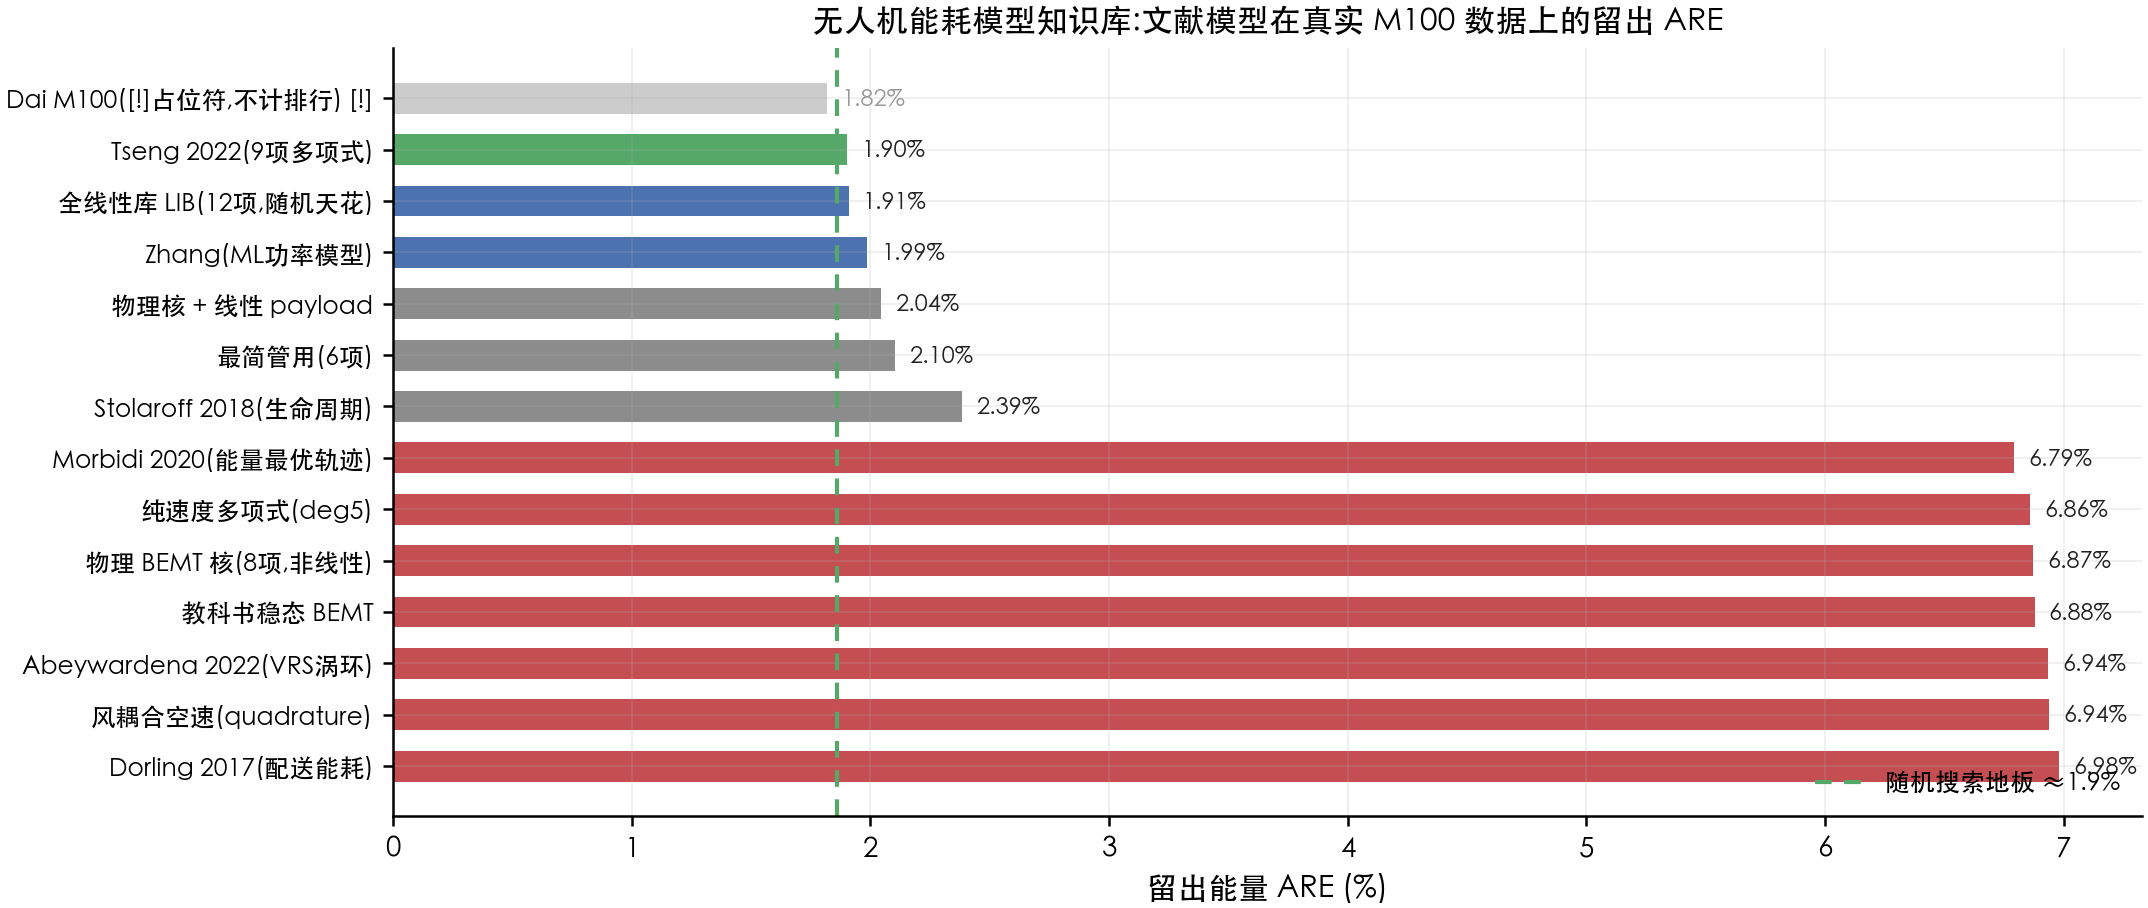
\includegraphics[width=\textwidth]{模型知识库排行榜.png}
\caption{Knowledge-base leaderboard: 14 literature models refit on the frozen M100
  evaluator (energy ARE, lower is better). Data-driven models dominate; physics forms stay
  6.7--7.0\%.}
\label{fig:zoo}
\end{figure*}

\begin{figure}[t]
\centering
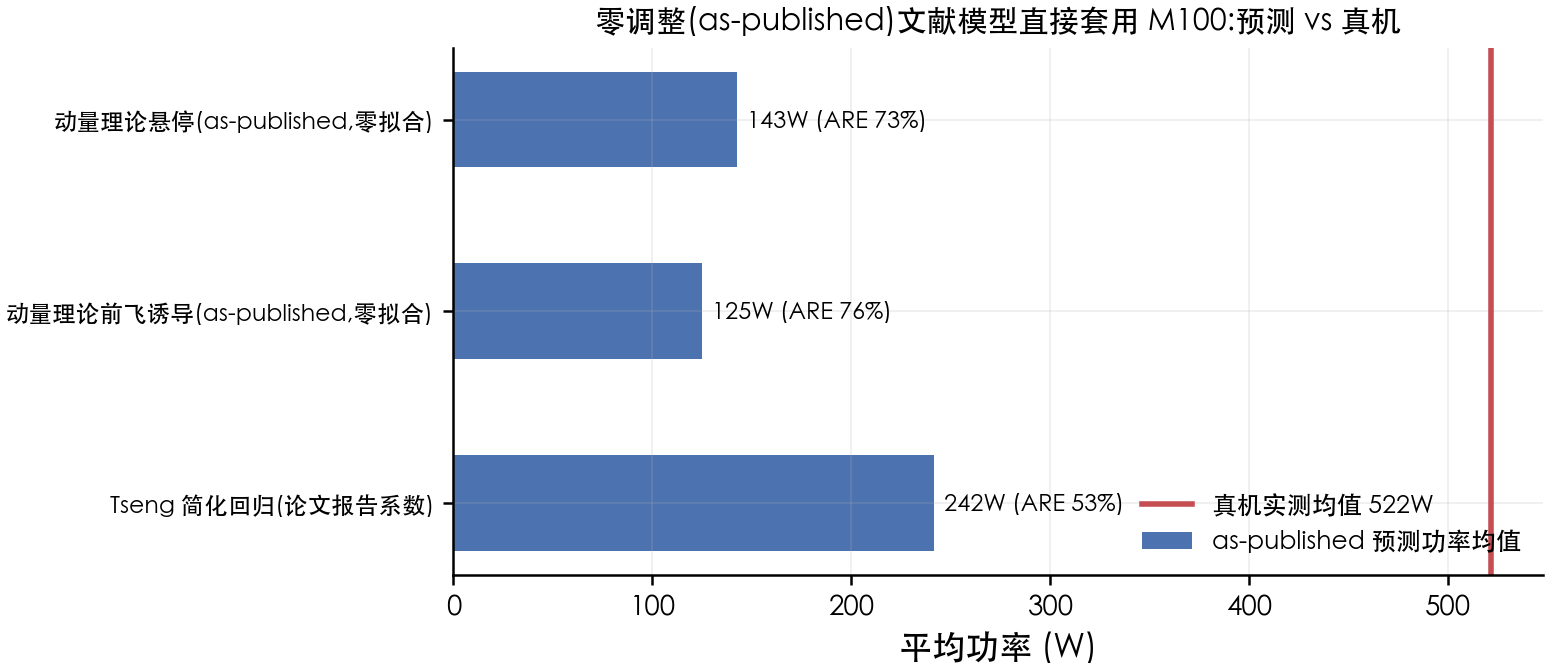
\includegraphics[width=0.9\linewidth]{as_published_vs_refit.png}
\caption{Zero-fit vs.\ refit. As-published models fail (energy ARE 53--76\%, predicted
  power far below measured 522\,W); refit recovers them to $\approx$2\%.}
\label{fig:asfit}
\end{figure}

\subsection{The cheat-proof loop}
\label{sec:exp-loop}
The loop starts from the knowledge-base winner (Tseng, 1.90\%) and converges at the data
floor. Instant-power analysis (Fig.~\ref{fig:instant}) shows why the \emph{planning}
result holds: at climb, textbook BEMT misses by $-131$\,W ($-20\%$); our loop is within
$\pm5\%$.

\begin{figure}[t]
\centering
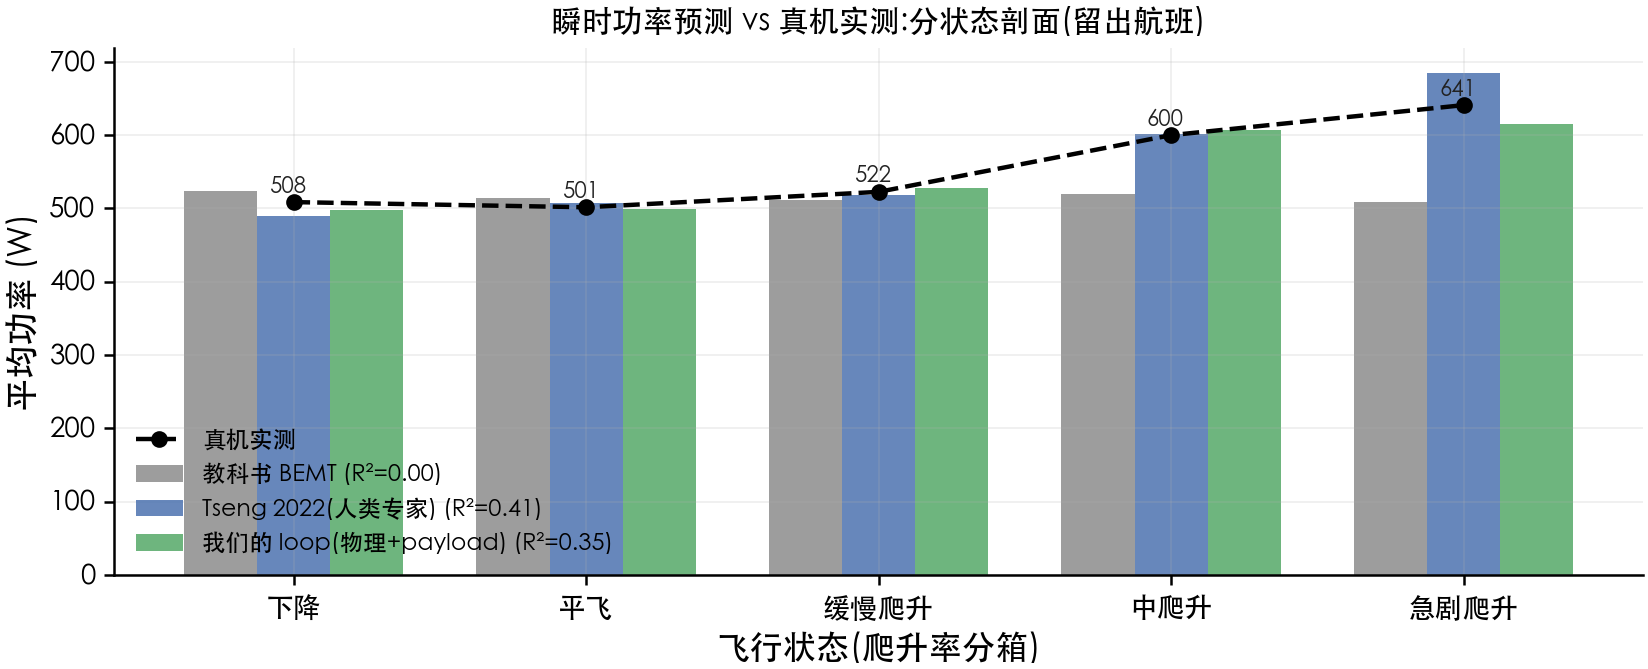
\includegraphics[width=0.9\linewidth]{瞬时功率误差.png}
\caption{Per-state instantaneous power error. At climb, textbook BEMT misses by $-13\%$
  to $-20\%$ ($-131$\,W at steep climb); our loop is within $\pm5\%$ on all climb states.}
\label{fig:instant}
\end{figure}

The safeguard ablations (\texttt{safeguard\_ablation.py}) show every mechanism is
load-bearing: the frozen ruler resists a gaming probe (2.13\% vs.\ honest 1.99\%); the
novelty gate demotes 2 of 3 ``discoveries'' to known prior art (Michel 2024, Nguyen 2017);
the external-search branch escapes a local-optimum basin (4.2\% $\rightarrow$ 1.9\% via
``add linear payload''); and the loop's value is domain-dependent. Fig.~\ref{fig:ablation}
summarizes the load-bearing mechanisms.

\begin{figure}[t]
\centering

\includegraphics[width=0.9\linewidth]{框架消融_局部最优.png}
\caption{Local-optimum escape: seven physics variants are stuck at $\approx$4.2--4.5\%
  (red basin); the external-search branch identifies ``add linear payload'' and reaches
  1.93\% (green)---the escape is load-bearing.}
\label{fig:ablation}
\end{figure}

\paragraph{Live demonstration of the val-discipline (loop iter 12).} A piecewise
hover/cruise model was \emph{better on all three held-out val seeds} ($\Delta
-0.006/-0.061/-0.014$ pp) but \emph{worse on the search split} (2.049\% vs.\ 1.991\%).
The protocol rejected it because search is the selector and val only a guard---a naive
pipeline would have kept it and overfit to the val split.

\subsection{Capability law and the Headroom Diagnostic}
\label{sec:exp-capability}
Two real endpoints: energy tie ($z=-0.35$) and planning win ($z=-2.38$, 8.1\%). One
controlled negative control: nominal-space inflation ($K=8\ldots200$) yields advantage
$\approx 0$. One decomposition: planning win = cross-space escape ($-382$ from code). One
synthetic third domain: low/high effective-dimension, mechanism confirmed.
Fig.~\ref{fig:twodom} (two-domain significance, negative control inset),
Fig.~\ref{fig:predobs} (prediction vs.\ observation), and
Fig.~\ref{fig:threedom} (three-domain summary) present these.

\begin{figure}[t]
\centering

\includegraphics[width=0.9\linewidth]{两域显著性.png}
\caption{Two-domain significance. Energy: loop $=1.86\%$ vs.\ random $1.87\pm0.03\%$,
  $z=-0.35$ (tie); inset = controlled negative control (nominal K inflation $\rightarrow$
  advantage $\approx 0$). Planning: loop $=2882$ vs.\ random $3135\pm106$, $z=-2.38$,
  $+8.1\%$, 0\% of random runs beat it.}
\label{fig:twodom}
\end{figure}

\begin{figure}[t]
\centering
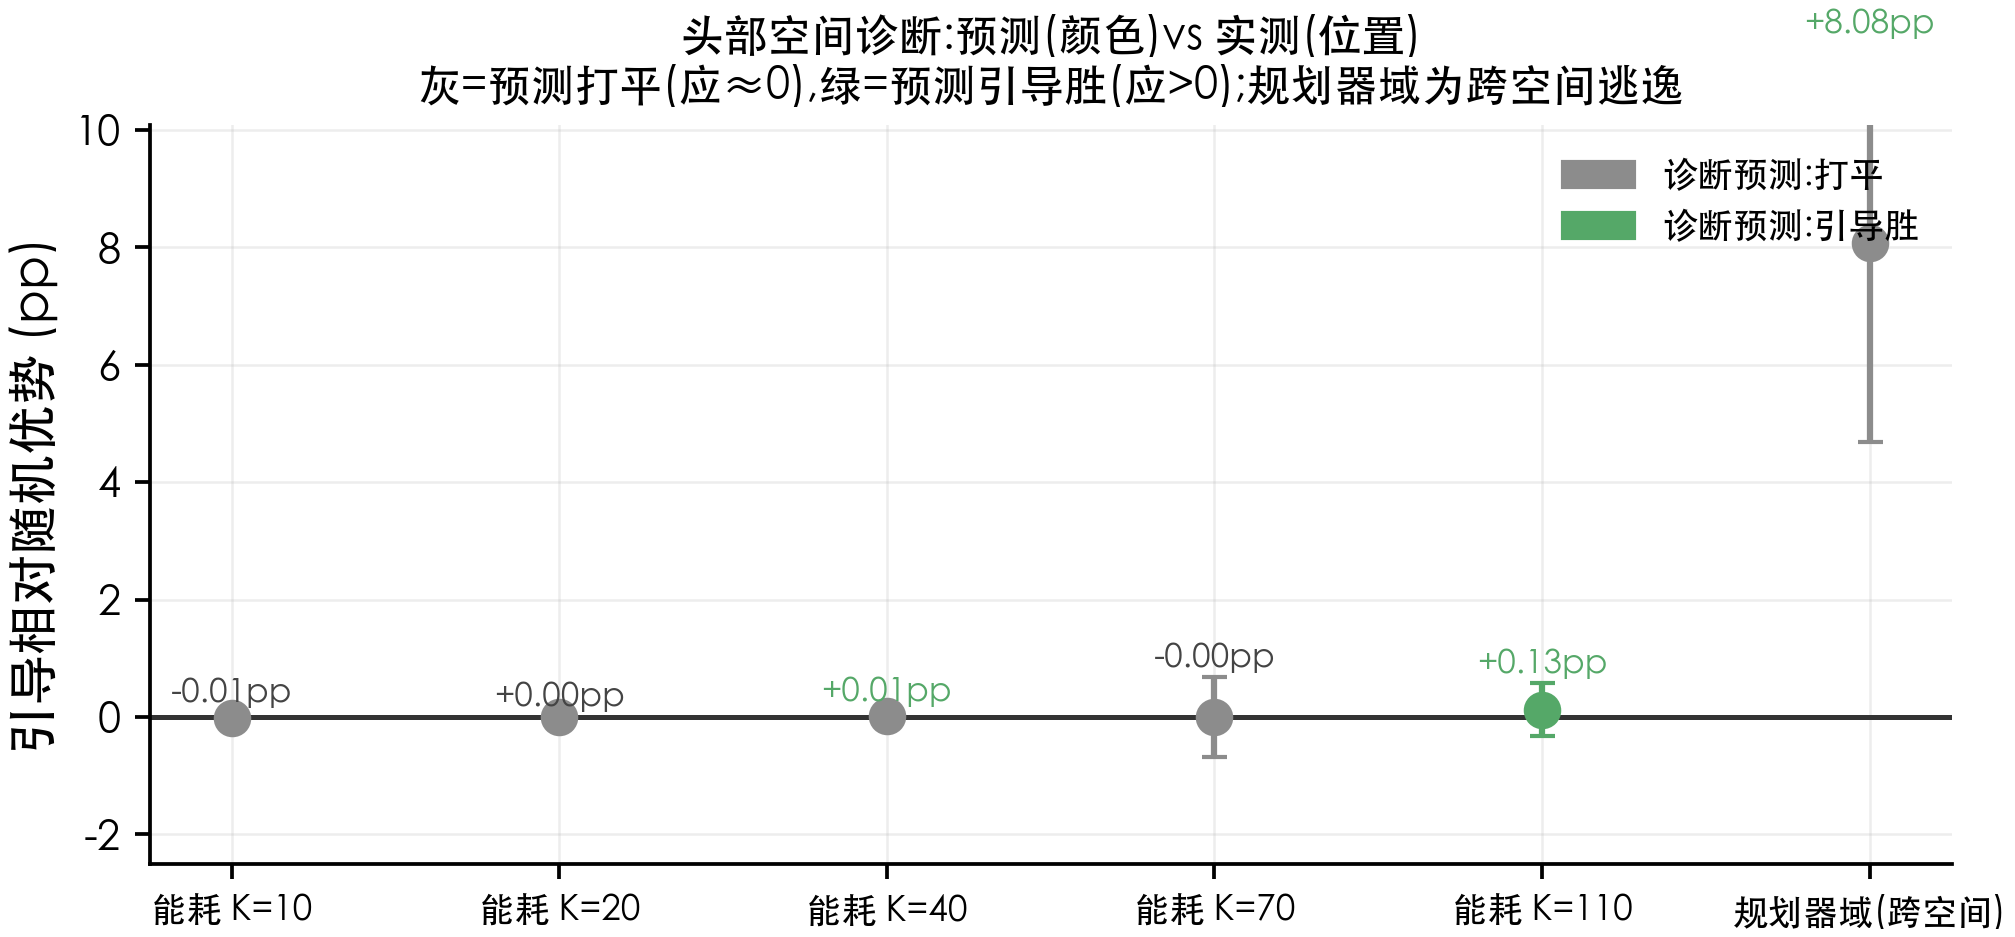
\includegraphics[width=0.9\linewidth]{头部空间诊断_预测vs实测.png}
\caption{Headroom diagnostic: prediction vs.\ observation. Color = predicted verdict
  (gray = tie, green = guided-wins); position = observed advantage (pp). All predictions
  match.}
\label{fig:predobs}
\end{figure}

\begin{figure*}[t]
\centering
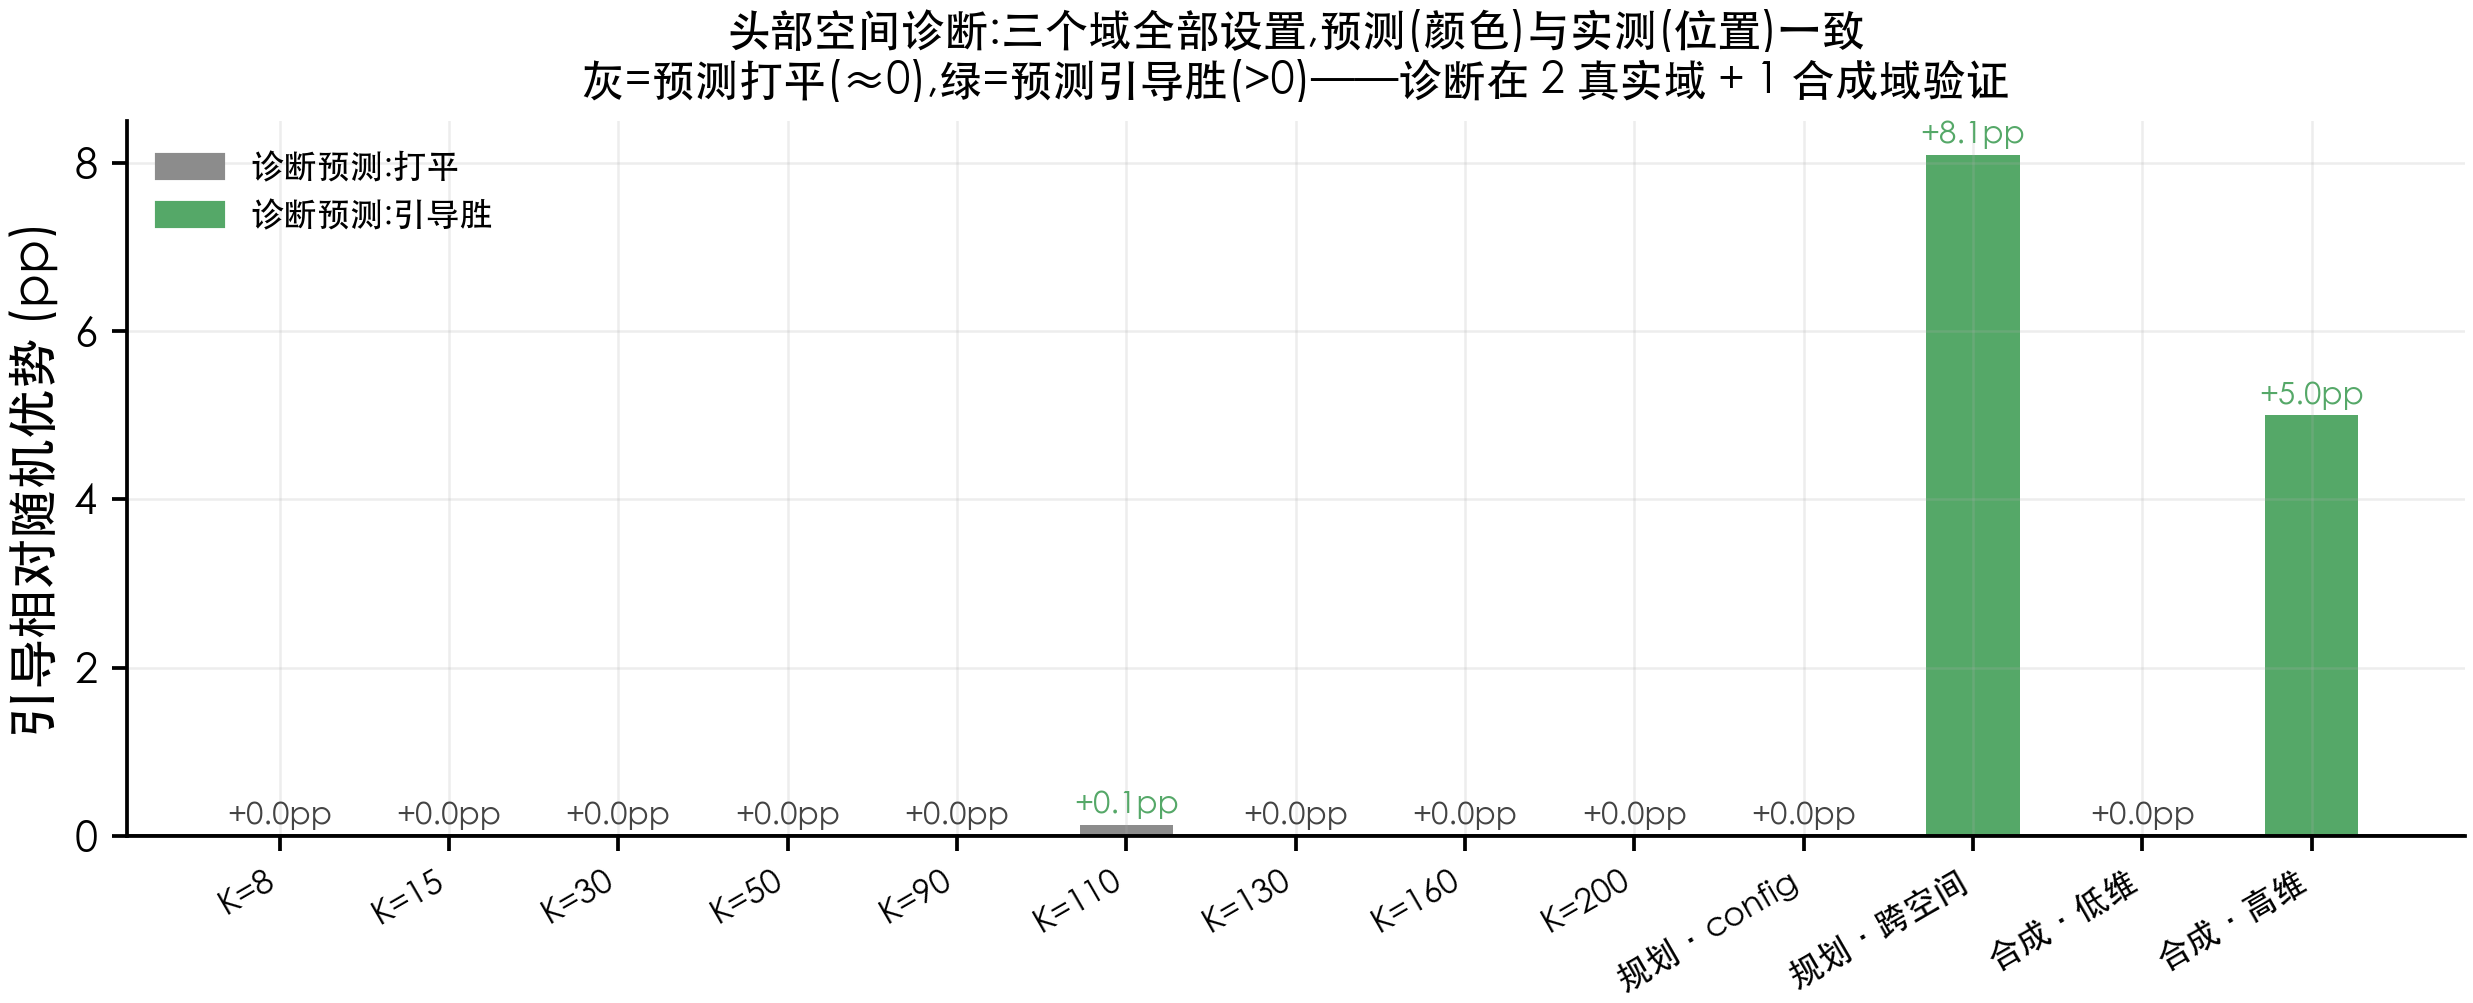
\includegraphics[width=0.85\textwidth]{头部空间诊断_三域验证.png}
\caption{Three-domain diagnostic validation: energy 9 K-levels (tie), planning
  config-tie + cross-space win, synthetic low/high effective-dim. Every prediction
  matches.}
\label{fig:threedom}
\end{figure*}

\subsection{Deployment value of the diagnostic}
\label{sec:exp-value}
Following the diagnostic as a decision rule is strictly better than defaulting to running
the loop: in the energy domain (predict tie) the knowledge-base start (1.90\%) beats the
loop's own product (1.93\%), so the ``skip'' advice saves the budget \emph{and} yields the
better model; in the planning domain the diagnostic detects the escapable code space and
investing pays ($+8.1\%$, $z=-2.38$). This is a concrete ``when to run autoresearch''
rule: \emph{skip in saturated spaces, invest where a higher-complexity space is
escapable.}

% =============================================================================
\section{Honest Capability Boundaries}
\label{sec:boundaries}
\begin{enumerate}
  \item Guided search does \textbf{not} beat random in the energy domain. That \emph{is}
    the finding, not a failure.
  \item Tseng is the same dataset's human result; we match (1.90 vs.\ 1.93), we do not
    claim to beat human modeling.
  \item Instantaneous power: kinematics explain $<40\%$ of variance; per-flight energy is
    the stable, plan-able quantity.
  \item Zero-fit transfer numbers include scale-mismatch for Tseng's simplified form---
    reported as approximate.
  \item The planning win is measured on a synthetic corridor; real-outdoor validation is
    future work.
\end{enumerate}

% =============================================================================
\section{Discussion}
\label{sec:disc}
\paragraph{Why nominal space size does not predict guided advantage.} Bergstra and the
NAS results suggest the lever is \emph{effective} dimensionality. Our controlled sweep
confirms it directly: inflating the nominal pool from 8 to 200 terms did not make guided
search pull ahead, because the real signal concentrates in a handful of terms.

\paragraph{Cross-space escape as the real lever.} Within a saturated config space the
loop ties random (3264 $\approx$ 3135), but the LLM can \emph{write code} (a smoother)
that random config search cannot reach. This is the measured, quantitative version of the
FunSearch/AlphaEvolve program-space claim.

\paragraph{Toward a principled answer to ``when does guided search help?''}
The two findings together resolve a tension in the autoresearch literature. FunSearch and
AlphaEvolve operate in program spaces so vast that guided search is clearly necessary;
Bergstra and the NAS literature show random search ties guided search in
low-effective-dimension spaces. Between these extremes, no prior work quantifies the
transition. Our controlled sweep (energy domain, nominal-space inflation does not help)
locates the ``random-ties'' regime precisely, and our cross-space decomposition locates
the ``guided-wins'' regime: the advantage appears exactly when the LLM can escape the
current (saturated) space into a higher-complexity one it can propose in. The headroom
diagnostic operationalizes this: it reads the spread/synergy signature of the search
space to predict, before spending budget, which regime the task is in. This is, to our
knowledge, the first measured account of the transition between these regimes, on real
hardware data.

% =============================================================================
\section{Conclusion}
\label{sec:conclusion}
We presented a trustworthy autoresearch protocol for noisy engineering domains,
instantiated on real UAV energy modeling and energy-aware planning, with a pre-loop
headroom diagnostic that correctly identifies when the loop is worth running. The
protocol is honest by construction: it reports ties and negative results, and every
safeguard is load-bearing by ablation. Its convergence matches a human expert on the same
data; its capability boundaries are measured, not asserted.

% =============================================================================
\section{Threats to Validity and Defenses}
\label{sec:threats}
\paragraph{T1: ``An LSTM beats your energy model by 72\% RMSE (Muli et al.\ \citep{muli2022}).''}
Our claim is not ``best energy model.'' It is ``trustworthy autoresearch protocol + a
diagnostic for when guided search helps.'' We match the human polynomial baseline (1.93\%
vs.\ 1.90\% per-flight energy ARE; the LSTM's 36 RMSE in \citep{muli2022} is per-sample, a
different quantity and a black box unusable as an interpretable planning cost).

\paragraph{T2: ``The headroom diagnostic is only validated in a few domains.''}
The diagnostic is a mechanism-based rule (utility spread + combination synergy), not a
fitted classifier---no parameters are trained on the outcome. It is validated at 9
controlled complexity levels in energy, at 2 planning settings, and in a synthetic third
domain with controlled effective dimension.

\paragraph{T3: ``The loop is net-negative in the energy domain.''}
That is precisely the point. The energy domain is a \emph{saturated} space; the honest
protocol---and the diagnostic---recognize this and stop. Our protocol's value is
\emph{knowing when not to run}, and the planning domain shows it \emph{knows when to
invest} ($+8.1\%$).

\paragraph{T4: ``The zero-fit benchmark is unfair to physics models.''}
That is the finding: platform-bound coefficients make zero-fit transfer fail, which is why
refit is a protocol stage rather than an assumption. The refit numbers (physics forms
still 6.7--7.0\%) show the failure is not only coefficient-bound.

\paragraph{T5: ``The planning domain is synthetic.''}
Accepted as a limitation. The energy-modeling instantiation uses real DJI M100 data; the
planning instantiation uses the standard kinodynamic simulator. Real-outdoor planning
validation is future work.

% =============================================================================
\section*{Implementation Details}
\label{app:impl}

\textbf{Data split.} 209 DJI M100 flights, flight-level 70/30 train/test split (no
cross-flight leakage). Search uses seeds 0,1,2; held-out validation uses seeds 5,6,7.
Held-out flights are never touched during search---they enter only for final evaluation.

\textbf{Evaluator.} Per-flight energy ARE = mean over held-out flights of
$|E_{\mathrm{pred}} - E_{\mathrm{true}}| / E_{\mathrm{true}}$, where $E = \int P\,dt$ with
$P = V\cdot|I|$ (on-board measurement). Feature columns are z-scored on the training
split; ridge regression with $\lambda = 10^{-4}\,\mathrm{tr}(X^\top X)/K$.

\textbf{Knowledge-base benchmark.} 14 models (\texttt{energy\_model\_zoo.py}), each refit
with the above ridge protocol; zero-fit models (\texttt{as\_published\_benchmark.py}) use
no fitting.

\textbf{Fair complexity sweep (\texttt{complexity\_scaling\_fair.py}).} Candidate pools of
size $K \in \{10,20,40,70,110\}$ (fine-grid 8--200 in the diagnostic probe); budget 30;
6 seeds; guided = single-term-utility-weighted sampling (softmax temperature 0.5),
random = uniform; both use the same subset-sampling action space. Advantage measured as
random $-$ guided (held-out ARE).

\textbf{Headroom diagnostic (\texttt{headroom\_diagnostic.py}, Algorithm~\ref{alg:headroom}).}
Single-term utilities on the search split; best-combination = median of best budget-30
random subsets over 5 seeds (median removes single-seed noise). Thresholds: tie iff
rel\_spread $> 0.3$ and headroom $< 0.05$.

\textbf{Planning significance (\texttt{planner\_significance.py}).} $R{=}12$ random
config searches $\times$ $B{=}15$ budget each, default smoother; loop = tuned config +
evolved smoother. Config space: step\_size $\in [1,5]$, max\_iterations $\in [3000,8000]$,
goal\_sample\_rate $\in [0.1,0.6]$, search\_radius $\in [3,7]$, use\_rrt\_connect random.
Score = \texttt{physics\_eval.evaluate(overrides, runs=3, seed0=0)["score"]}. Cross-space
decomposition: config-only loop = tuned config + default smoother (3264); full loop adds
evolved smoother (2882).

\textbf{Safeguard ablations (\texttt{safeguard\_ablation.py}).} Frozen-ruler: overfit probe
(35 spurious terms) vs.\ honest models on search ARE. Novelty gate: 5 planning hypotheses
adjudicated with vs.\ without literature gate. Local-optimum: 7 physics variants vs.\
external-search escape.

All seeds are fixed; every number in the paper traces to the committed JSONs.

% =============================================================================
\section*{Acknowledgements}
% TODO: add funding/grant info before submission.
We thank the anonymous reviewers of earlier drafts for comments that improved the
honest-boundary framing. The DJI M100 dataset is from Rodrigues et al., Scientific
Data 2021 (CC-BY).

\section*{Author Contributions}
B.W. designed the protocol and diagnostic, ran the experiments, and wrote the paper.
L.Z. supervised the research and contributed to the experimental design and the
honest-boundary framing.

% =============================================================================
\begin{thebibliography}{99}

\bibitem[Romera-Paredes et al.(2024)]{funsearch}
B.~Romera-Paredes et al.
Mathematical discoveries from program search with large language models.
\emph{Nature}, 625:468--475, 2024.

\bibitem[Novikov et al.(2025)]{alphaevolve}
A.~Novikov et al.
AlphaEvolve: A coding agent for scientific and algorithmic discovery.
\emph{DeepMind}, 2025.

\bibitem[Ma et al.(2024)]{eureka}
Y.~J. Ma et al.
Eureka: Human-level reward design via coding large language models.
\emph{ICLR}, 2024.

\bibitem[Lu et al.(2024)]{aiscientist}
C.~Lu et al.
The AI Scientist: Towards fully automated open-ended scientific discovery.
\emph{arXiv:2408.06292}, 2024.

\bibitem[Beel et al.(2025)]{beel2025}
J.~Beel, B.~Kan, and M.~Baumgart.
Hidden pitfalls of AI Scientist systems.
\emph{ACM SIGIR Forum}, 2025. arXiv:2502.14297.

\bibitem[Jablonka et al.(2026)]{corral2026}
K.~M. Jablonka et al.
Corral: A benchmark of 25k agent runs for scientific reasoning.
\emph{arXiv}, 2026.

\bibitem[Position paper(2026)]{falsify2026}
Falsify, don't just discover: A position paper on automated falsification for
AI-driven science.
\emph{arXiv}, 2026.

\bibitem[Case study(2026)]{foureattempts2026}
Why LLMs aren't scientists yet: Lessons from four autonomous research attempts.
\emph{arXiv:2601.03315}, 2026.

\bibitem[Nature MI Editorial(2026)]{naturemi2026}
Multi-agent AI systems need transparency.
\emph{Nature Machine Intelligence}, 2026.

\bibitem[Liu et al.(2024)]{aigs}
J.~Liu et al.
AI-generated science from AI-powered automated falsification.
\emph{arXiv:2411.01710}, 2024.

\bibitem[Rodrigues et al.(2021)]{rodrigues2021}
T.~A. Rodrigues et al.
DJI M100 UAV energy dataset.
\emph{Scientific Data}, 8:219, 2021.

\bibitem[Muli et al.(2022)]{muli2022}
C.~Muli, S.~Park, and M.~Liu.
A comparative study on energy consumption models for drones.
\emph{arXiv:2206.01609}, 2022.

\bibitem[Abeywardena et al.(2022)]{abeywardena}
D.~Abeywardena et al.
Modelling power consumptions for multi-rotor UAVs.
\emph{arXiv:2209.04128}, 2022.

\bibitem[Dorling et al.(2017)]{dorling}
K.~Dorling et al.
Vehicle routing problems for drone delivery.
\emph{IEEE T-SMC}, 47(1), 2017.

\bibitem[Stolaroff et al.(2018)]{stolaroff}
J.~K. Stolaroff et al.
Energy use and life cycle assessment of drones for package delivery.
\emph{Nature Communications}, 9:409, 2018.

\bibitem[Morbidi et al.(2020)]{morbidi}
F.~Morbidi et al.
Energy-efficient trajectory generation for a hexarotor.
\emph{IEEE Trans. Robotics}, 2020.

\bibitem[Bergstra and Bengio(2012)]{bergstra2012}
J.~Bergstra and Y.~Bengio.
Random search for hyper-parameter optimization.
\emph{JMLR}, 13:281--305, 2012.

\bibitem[Wang et al.(2013)]{rembo}
Z.~Wang, M.~Zoghi, F.~Hutter, D.~Matheson, and N.~de~Freitas.
Bayesian optimization in high dimensions via random embeddings.
\emph{IJCAI}, 2013.

\bibitem[Sciuto et al.(2019)]{sciuto2019}
C.~Sciuto et al.
On the importance of the search space in NAS.
\emph{arXiv:1902.04158}, 2019.

\bibitem[Michel et al.(2024)]{michel2024}
A.~Michel et al.
Energy-optimal waypoint UAV missions.
\emph{arXiv:2410.17585}, 2024.

\bibitem[Nguyen and Au(2017)]{nguyen2017}
N.~Nguyen and T.~C. Au.
Finding minimum-cost drone delivery route for UAV.
\emph{AAMAS}, 2017.

\bibitem[LAENet(2025)]{laenet}
LAENet: LLM-designed UAV energy-minimization reward.
\emph{arXiv:2505.21045}, 2025.

\end{thebibliography}

\end{document}
